\section{Auswertung}

    \subsection{Hysteresekurve einer Nickel-Eisen-Legierung (5000 H2)}
        \label{sec:H2}
    PERMENORM 500 H2 ist eine Nickel-Eisen-Legierung, welche aufgrund ihrer hohen Permeabilität und geringen Koerzitivfeldstärke
    häufig in Transformatoren und Induktivitäten verwendet wird. \\
    Die experimentell aufgenommene Hysteresekurve ist in Abbildung \ref{fig:5000H2_Hysteresekurve} dargestellt.
    Sie zeigt den charakteristischen Verlauf eines weichmagnetischen Werkstoffs, bei welchem sowohl Remanenz als auch
    Koerzitivfeldstärke gering sind.
    \begin{figure}[H]
        \centering
        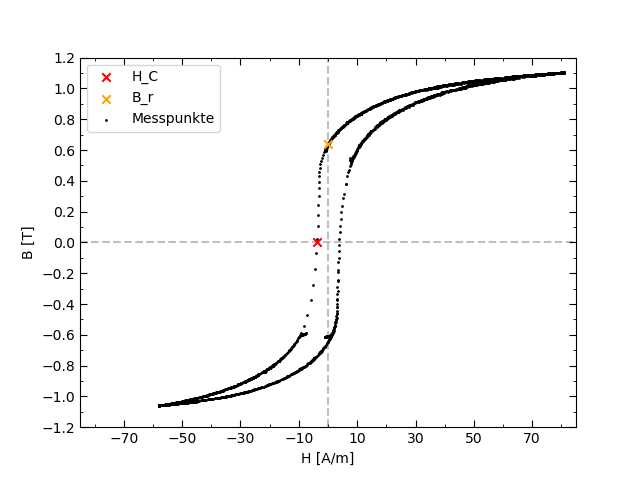
\includegraphics[width=0.45\textwidth]{../Images/Hyster1.png}
        \caption{Aufgenommene Hysteresekurve der Nickel-Eisen-Legierung PERMENORM 5000 H2.}
        \label{fig:5000H2_Hysteresekurve}
    \end{figure}
    Die aus der Messkurve bestimmten Werte sind:
    \begin{equation*}
        B_r = 0.6374 \pm 0.0025 \, T \quad , \quad H_c = 3.86 \pm 0.12 \, A/m
    \end{equation*}
    Zur Bestimmung der Sättigungsinduktion $B_s$ wurde ein erweiterter Messbereich verwendet (vlg. Abb. \ref{fig:Saett1}).
    \begin{figure}[H]
        \centering
        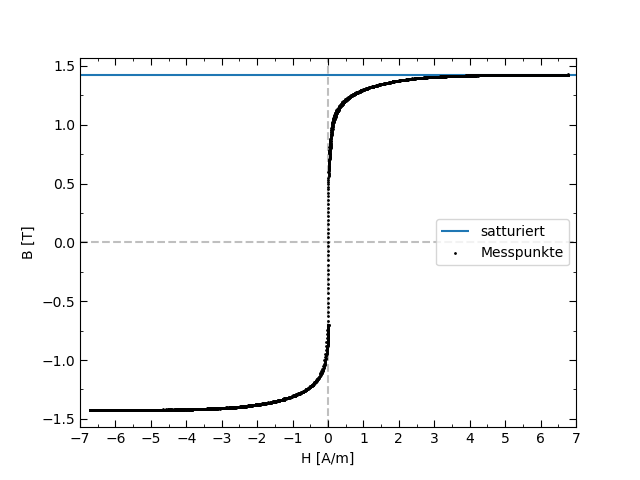
\includegraphics[width=0.45\textwidth]{../Images/Hyster1_Saett.png}
        \caption{Erweiterte Messung zur Bestimmung der Sättigungsinduktion der Nickel-Eisen-Legierung PERMENORM 5000 H2.}
        \label{fig:Saett1}
    \end{figure}
    Für hohe Feldstärken $ |H| \geq 1500 A/m$ kann angenommen werden, dass sich das Material 
    im Bereich nachezu konstanter Magnetisierung befindet, sodass der verbleibende lineare Anstieg der Flussdichte direkt dem
    äußeren Feld zugeordnet werden kann. \\
    Durch lineare Regression in diesem Bereich (vgl. Abb. \ref{fig:Saett1}) und Extrapolation auf $ H = 0$ lässt sich die Sättigungsinduktion
    bestimmen: 
    \begin{equation*}
        B_s = 1.58323 \pm 0.00010 \, T
    \end{equation*}
    \textcolor{red}{Hier noch mag. Feldkonstante?}
    \\
    Die Literaturwerte für PERMENORM 5000 H2 sind \cite{Permenorm}:
    \begin{equation*}
         B_{s,lit} = 1.55 \, T \quad , \quad H_{c,lit} = 5 \, A/m
    \end{equation*}
    Die gemessenen Werte stimmen somit nicht innerhalb der Unsicherheiten mit den Literaturwerten überein.
    Neben der unvollständigen Sättigung des Materials könnte dies auf materialspezifische Abweichungen im Legierungsverhältnis
    zurückzuführen sein. \\
    Aufgrund seiner geringen Koerzitivfeldstärke zählt PERMENORM 5000 H2 zu den weichmagnetischen Werkstoffen und ist daher für Dauermagnetanwendungen ungeeignet.
    Die leichte Ummagnetisierbarkeit und geringe Hysteresekurve machen das Material jedoch gut geeignet für Anwendungen bei den ein häufiger
    Magnetisierungswechsel auftritt, wie z.B. in Transformatoren, Drosselspulen oder magnetischen Abschirmungen.

    \subsection{Hysterese von Holz}
    Holz besitzt als diamagnetischer Werkstoff \cite{Holz} keine nennenswerte Hysteresekurve. Daher ist ein linearer Zusammenhang zwischen
    magnetischer Feldstärke $H$ und magnetischer Flussdichte $B$ zu erwarten. 
    Die Steigung dieser Geraden entspricht der Permeabilität des Materials: $ \frac{dB}{dH} = \mu_0 \mu_r $.\\
    In Abb. \ref{fig:Holz}


    \subsection{Hysteresekurve eines Eisenkerns}
    Die Messung der Hysteresekurve eines Flachstahs wurde analog zu Abschnitt \ref{sec:H2} durchgeführt.
    \begin{figure}[h]
        \centering
        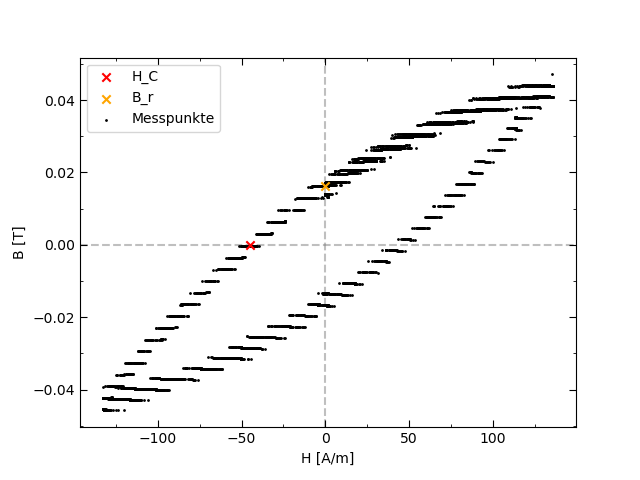
\includegraphics[width=0.45\textwidth]{../Images/Hyster3.png}
        \caption{Aufgenommene Hysteresekurve eines Eisenkerns.}
        \label{fig:Eisen_Hysteresekurve}
    \end{figure}
    Aus den jeweiligen Achsenschnittpunkten wurde die Remanenz $B_r$ und die Koerzitivfeldstärke $H_c$ bestimmt:
    \begin{equation*}
        B_r = 0.01620 \pm 0.00012 \, T \quad , \quad H_c = 45.13 \pm 0.44 \, A/m
    \end{equation*}
    Der Energieverlust wird mithilfe Gl. \ref{eq:Energieverlust} bestimmt:
    \textcolor{red}{Wert}
    
    Des weiteren wurde die Irreversibilität der Magnetisierung durch Richtungsänderung analysiert.
    Hierzu wurde zuerst ein vollständiger Hystereseverlauf aufgezeichnet, anschließend wurde bei erneutem
    Durchlaufen an zwei Stellen am abnehmenden Zweig die Richtung durch Erhöhen der magnetischen Feldstärke umgekehrt.
    Dadurch entstehen innere Hystereseschleifen (vgl. Abb. \ref{fig:Irreversibilitaet}), welche die selbe Durchlaufrichtung wie die Hystereseschleife hat.
    \begin{figure}[H]
        \centering
        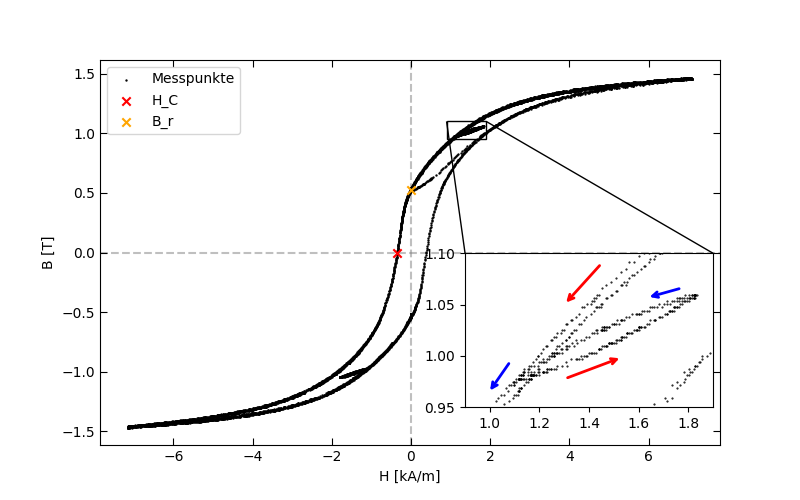
\includegraphics[width=0.45\textwidth]{../Images/Hyster3_irre.png}
        \caption{Untersuchung der Irreversibilität der Magnetisierung eines Eisenkerns durch Richtungsänderung.}
        \label{fig:Irreversibilitaet}
    \end{figure}
    Das Prinzip der inneren Hystereseschleifen lässt sich auch dazu verwenden, den Spulenkern zu entmagnetiseiert. Hierzu wird
    das maximal eingestellte Magnetfeld nach jeder Spannungsumpolung verringert, wodurch sich die Hystereseschleife dem Nullpunkt
    spiralartig nähert. Das ist in Abb. \ref{fig:Entmagnetisierung} dargestellt.
    \begin{figure}[H]
        \centering
        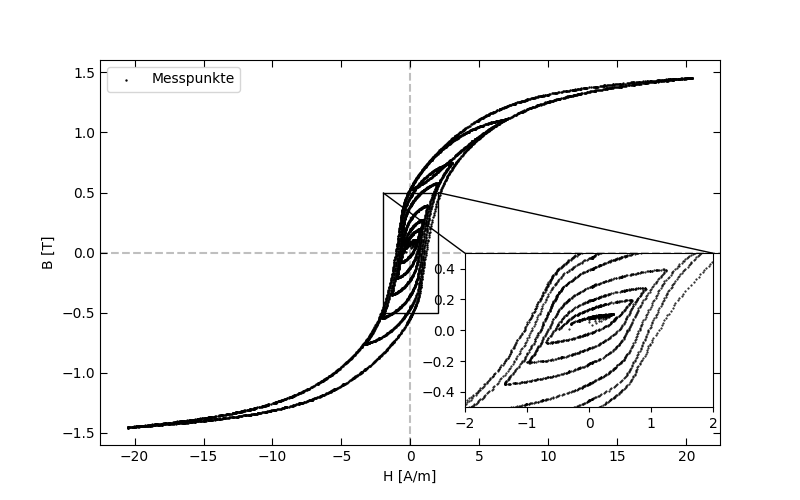
\includegraphics[width=0.45\textwidth]{../Images/Hyster3_entmag.png}
        \caption{Entmagnetisierung eines Eisenkerns durch sukzessive Verringerung des maximalen Magnetfeldes nach jeder Umpolung.}
        \label{fig:Entmagnetisierung}
    \end{figure}
    Für die vollständige Entladung darf das Magnetfeld erst nach Erreichen der Koerzitivfeldstärke umgepolt
    werden, sodass die Hysteresekurve im Nullpunkt endet. Dies wurde händisch nicht erreicht, wordurch eine Restmagnetisierung bleibt.

    \subsection{Hysteresekurve einer Nickel-Eisen-Legierung (5000 Z)}
        \label{sec:Z}
    PERMENORM 5000 Z ist eine weitere Nickel-Eisen-Legierung, deren magnetische Eigenschaften analog zu denen von
    PERMENORM 5000 H2 in Abschnitt \ref{sec:H2} untersucht wurden. \\
    \begin{figure}[h]
        \centering
        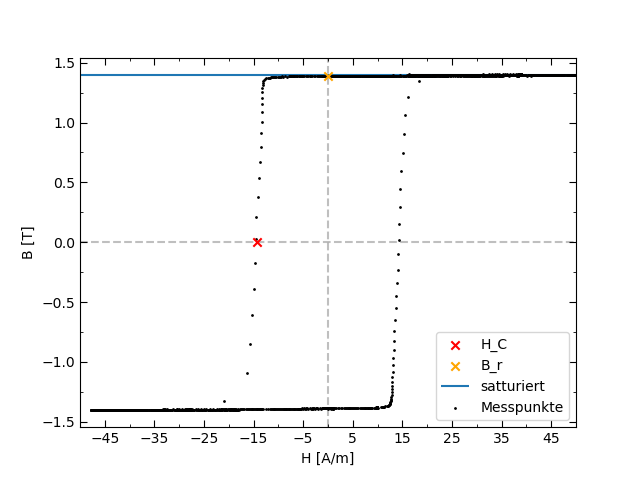
\includegraphics[width=0.45\textwidth]{../Images/Hyster2.png}
        \caption{Aufgenommene Hysteresekurve der Nickel-Eisen-Legierung PERMENORM 5000 Z.}
        \label{fig:5000Z_Hysteresekurve}
    \end{figure}
    Aus den jeweiligen Achsenschnittpunkten wurde wieder die Remanenz $B_r$ und die Koerzitivfeldstärke $H_c$ bestimmt:
    \begin{equation*}
        B_r = 1.38854 \pm 0.00024 \, T \quad , \quad H_c = 14.41 \pm 0.22 \, A/m
    \end{equation*}
    Die Sättigungsinduktion wurde wieder durch Extrapolation einer linearen Regression im Bereich hoher Feldstärken $|H| \geq 60 A/m$
    bestimmt:
    \begin{equation*}
        B_s = 1.55401 \pm 0.00015 \, T
    \end{equation*}
    Die kleine Koerzitivfeldstärke von PERMENORM 5000 Z deutet ebenfalls auf einen weichmagnetischen Werkstoff hin.
    Aufgrund der geringen Ummagnetisierungsverluste eignet sich die Legierung gut für Anwendungen 
    mit häufigem Magnetisierungswechsel, wie z.B. in Transformatoren oder Induktivitäten. \\
    Leider finde ich keine Datenblatt für PERMENORM 5000 Z, um die gemessenen Werte mit den Literaturwerten zu vergleichen.
    
    \subsection{Vergleich der Messergebnisse}
    \subsubsection{Ummagnetisierungsverluste}    
    \subsubsection{Hysteresekurven im Vergleich}
    Die Hysteresekurven der Fe-Ni-Legierungen weisen schmale Schleifen mit niedriger Koerzitivfeldstärke auf.
    Das ist charakteristisch für weichmagnetische Werkstoffe, welche sich durch geringe Ummagnetisierungsverluste
    auszeichnen. \\
    Im Vergleich dazu zeigt der Eisenkern eine deutlich breitere Hystereseschleife mit höherer Koerzitivfeldstärke,
    was auf höhere Ummagnetisierungsverluste und eine stärkere Remanenz hinweist. Daraus lässt sich folgern, dass der Eisenkern
    ein hartmagnetisches Material ist. \\